\chapter{Experimental work and results in mixed mode}
\label{Chapter2}

\section{Introduction}

In this section, the results obtained in mixed mode I+II are presented. The decoupling of the modes has allowed to obtain the share of mode I and II. The imposed displacement compliance method has been used to calculate the different energy release rates. The deformation maps, force vs Crack Tip Opening curves, and energy release rate vs crack length for different angles are presented below. It was decided to use only method 1 to measure the crack length as this method is more accurate than method 1. The values of the $G_\text{I} - G_\text{II}$ difference are also given. The calculation of the difference is intended to show the behaviour and evolution of the two modes with respect to the variation of the angle.

\section{Experimental set-up}

In the mixed mode I+II experiments, the camera-lens system was adjusted to match the orientation of the Arcan specimen and fixture, as shown in Figure \ref{fig:Setup15°}. This setup allowed for the direct projection of crack opening values along the $x$ and $y$ axes. Similarly, the force was projected along the $x$ and $y$ axes, as illustrated in Figure \ref{fig:fig37bis}.

\begin{figure}[htp]
	\centering
	\includegraphics[width=16cm]{Setup15°}
	\caption{Experimental set-up.}
	\label{fig:Setup15°}
\end{figure}

\section{Results}

\subsection{Strain fields}

Figure \ref{fig:Strain_def_mixedmode} presents the strain fields ($\varepsilon_{yy}$) for the two tilt angles (15° and 30°) of the specimen in mixed mode. Unfortunately, due to limited availability of specimens, results for the 45° tilt angle were not obtained. These strain maps are provided in terms of $x$ (pixels) and $y$ (pixels) coordinates. The progressive advancement of the crack can be clearly observed in these deformation maps. Although the crack path may not be perfectly straight, there is no apparent change in its direction. Consistent with the findings in Chapter 3, the crack propagation aligns with the orientation and inclination of the fibres.

\begin{figure}[htp]
	\centering
	\begin{tabular}{c}
		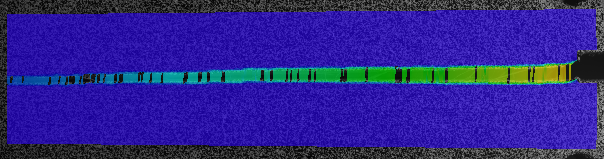
\includegraphics[width=8cm]{e15e2} \\
		e15e2 deformation map \\
		\\
		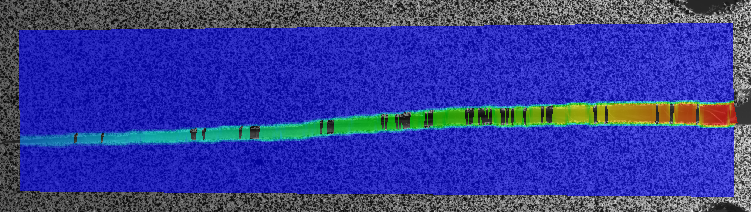
\includegraphics[width=8cm]{e30e3} \\
		e30e3 deformation map \\
		\\
		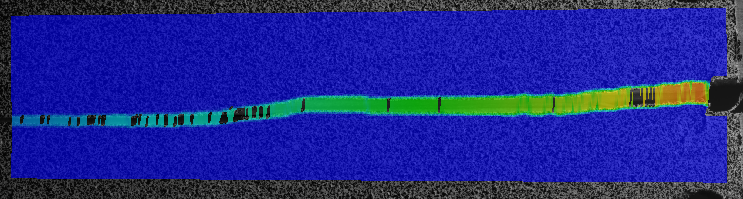
\includegraphics[width=8cm]{e30e5} \\
		e30e5 deformation map \\
	\end{tabular}
	\caption{Typical deformation map ($\epsilon$yy) obtained with DIC for mixed mode.}
	\label{fig:Strain_def_mixedmode}
\end{figure}

Similar to the previous chapter, the accuracy of crack length curves was confirmed by examining the $\varepsilon_{yy}$ strain fields. The crack tip can be visually identified on the strain maps, allowing for visual verification. Figures \ref{fig:e15e1_graphicread} and \ref{fig:e30e2_graphicread} depict the verification process for e15e1 and e30e2, respectively, through graphic reading. It appears that the crack length has been accurately estimated for each stage using method 1.

\begin{figure}[htp]
	\begin{minipage}[c]{.46\linewidth}
		\centering
		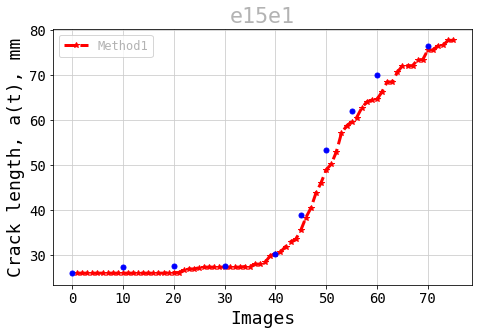
\includegraphics[width=8cm]{e15e1_graphicread}
		\caption{Crack tip by graphic reading e15e1.}
		\label{fig:e15e1_graphicread}
	\end{minipage}
	\hfill%
	\begin{minipage}[c]{.46\linewidth}
		\centering
		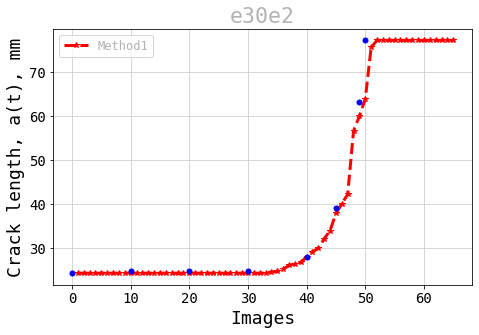
\includegraphics[width=8cm]{e30e2_graphicread}
		\caption{Crack tip by graphic reading e30e2.}
		\label{fig:e30e2_graphicread}
	\end{minipage}
\end{figure}

\subsection{Load versus crack tip opening displacement}

Figure \ref{fig:CTOD15} shows the evolution of the load as a function of the crack tip opening displacement for 15° specimens. For all the specimens, when a sudden drop in $P$ is observed, signifying the complete failure of the material, the values along the $x$ axis are less than 0.15 mm and of the order of 0.5 to 1.1 mm along the $y$ axis.

\begin{figure}[H]
	\centering
	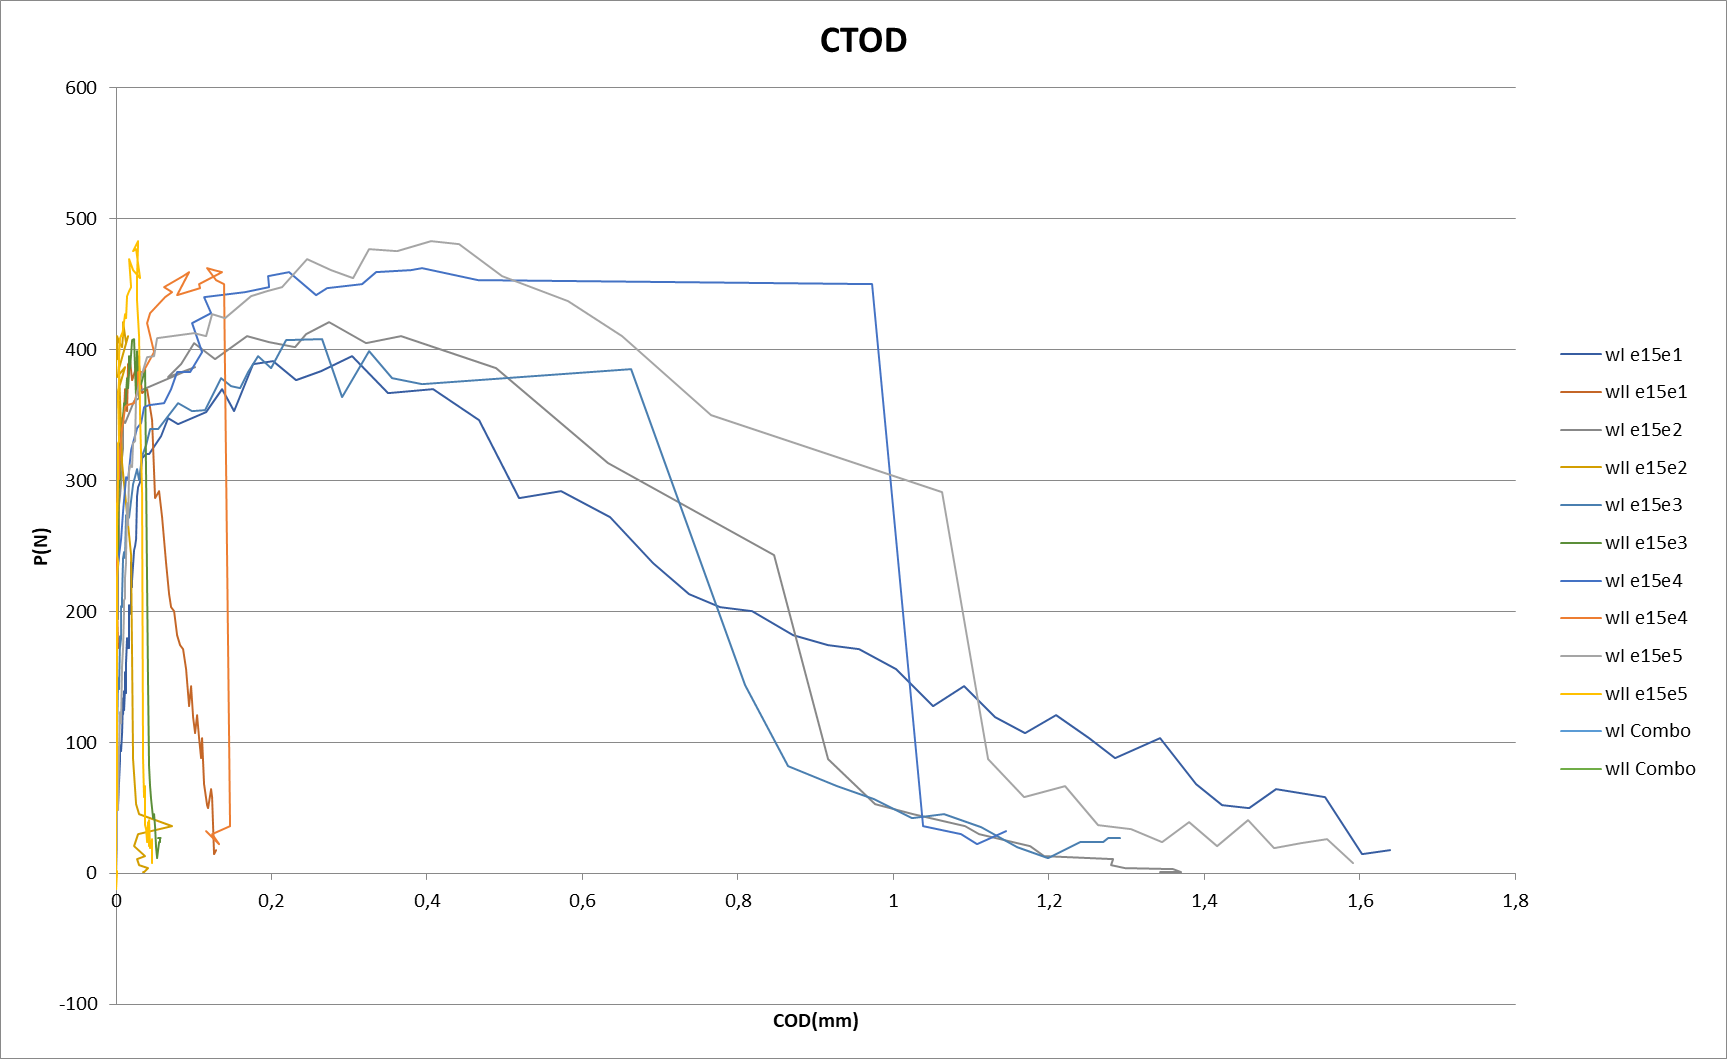
\includegraphics[width=15cm]{CTOD15}
	\caption{Evolution of the force as a function of the crack opening for 15° inclination.}
	\label{fig:CTOD15}
\end{figure}

Figure \ref{fig:CTOD30} shows the load curves as a function of the crack opening displacement for 30° specimens. As can be seen, the crack opening along $x$ for all the specimens tested is less than 0.11 mm. For the crack opening along $y$ when a sudden drop in $P$ is observed, the values are of the order of 0.4 to 1.1 mm.
We can also see that the CTOD of e30e2 does not have the expected shape. After the image 53 of 66, the CTOD is not recorded correctly. However, this is of no real importance as $P$ decreases sharply at stage 49, so it has no impact on the calculation of $G_\text{Imax}$.

\begin{figure}[H]
	\centering
	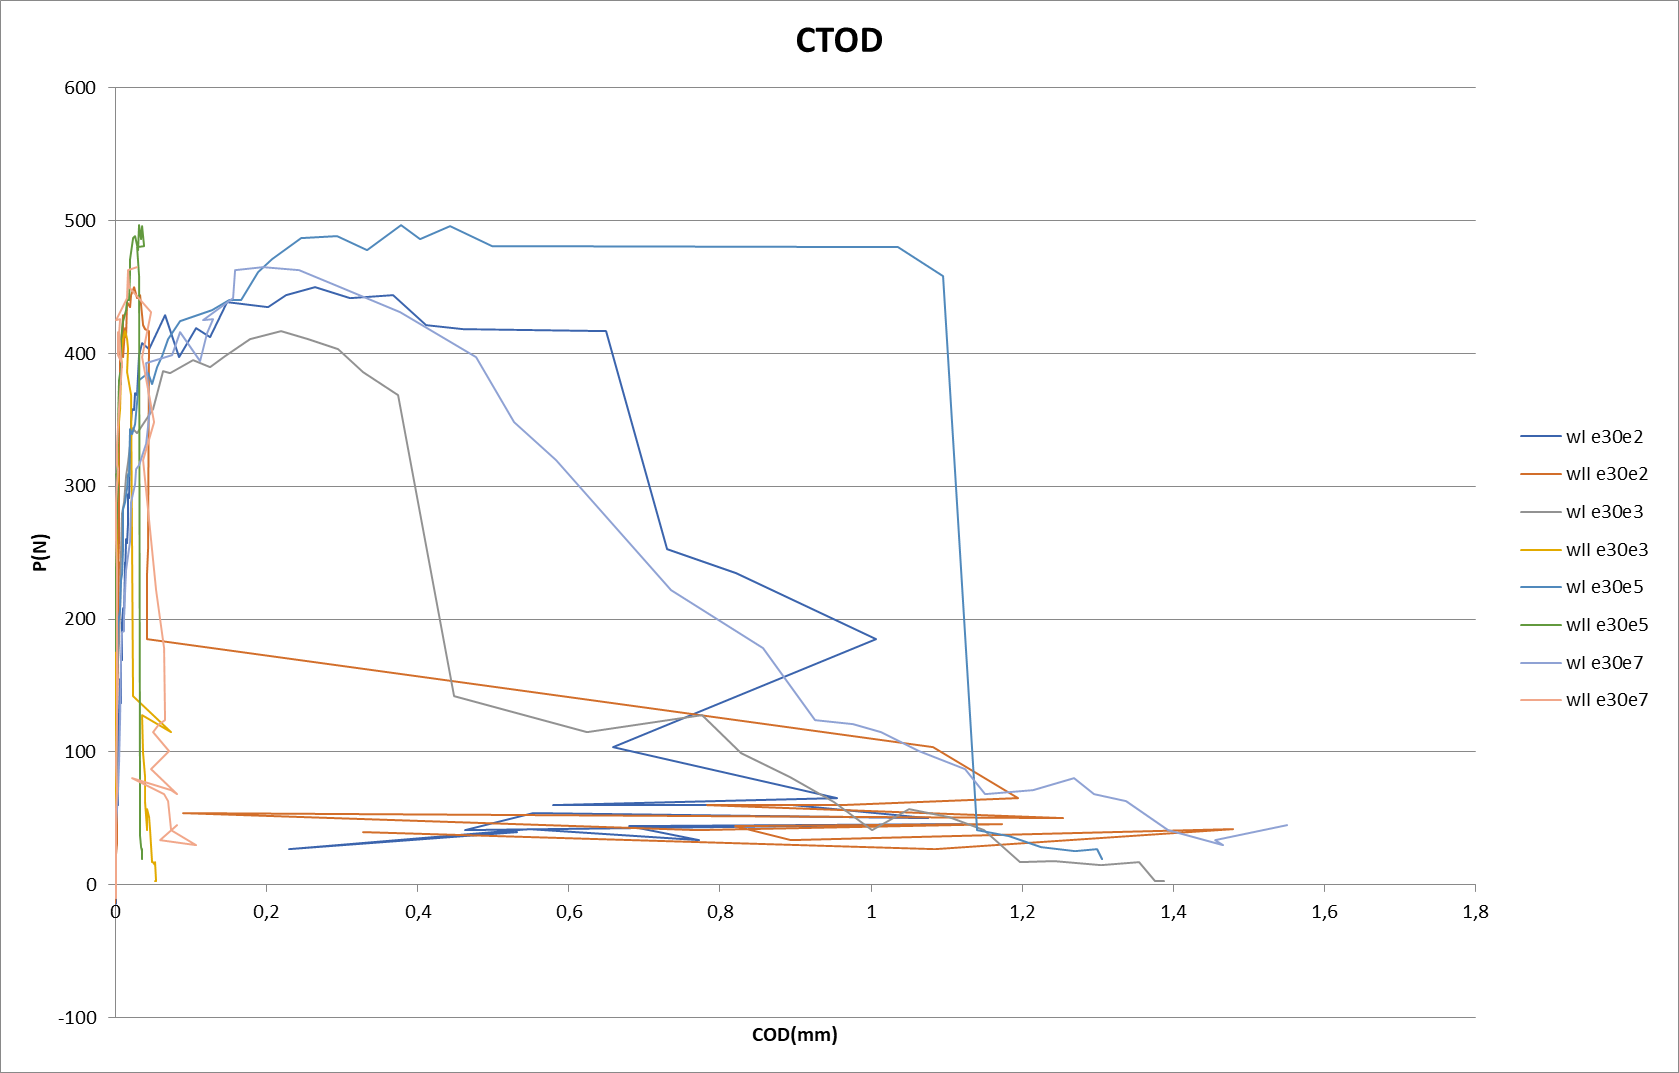
\includegraphics[width=15cm]{CTOD30}
	\caption{Evolution of the force as a function of the crack opening for 30° inclination.}
	\label{fig:CTOD30}
\end{figure}

We can say that for 15° and 30° angles the crack openings along the $x$-axis are negligible compared to those along the $y$-axis.

\subsection{Crack length curves}

All the crack length curve in function of displacement in mixed mode are shown in figure \ref{fig:crack_15} and \ref{fig:crack_30}. 
There are, as expected, different plateaus for the crack length. The crack length increases gradually and continuously before rupture. It is interesting to examine all the crack length propagation plots.  The curves are all more or less the same shape, and the crack ends at roughly the same length. What differs is the stage at which the crack begins to propagate. There are no major differences in crack length when you switch from mode I to mixed mode.

\begin{figure}[htp]
	\centering
	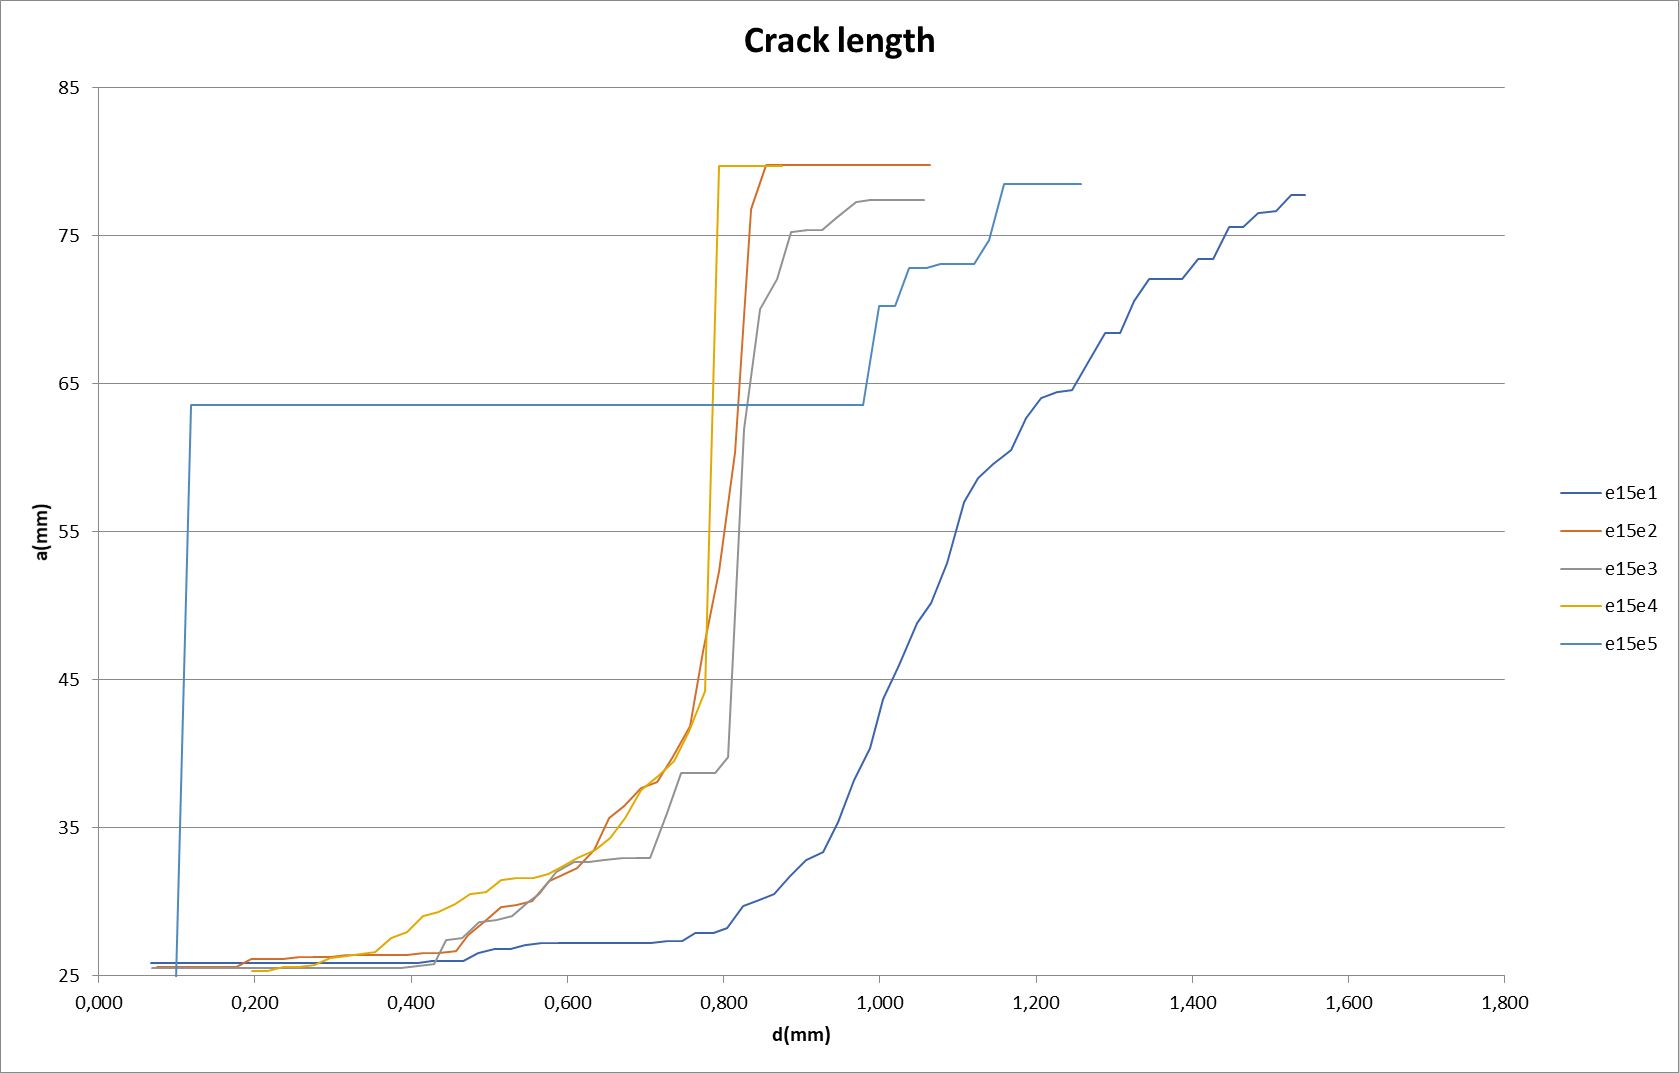
\includegraphics[width=13cm]{crack_15}
	\caption{Crack length evolution for 15° specimens.}
	\label{fig:crack_15}
\end{figure}

\begin{figure}[htp]
	\centering
	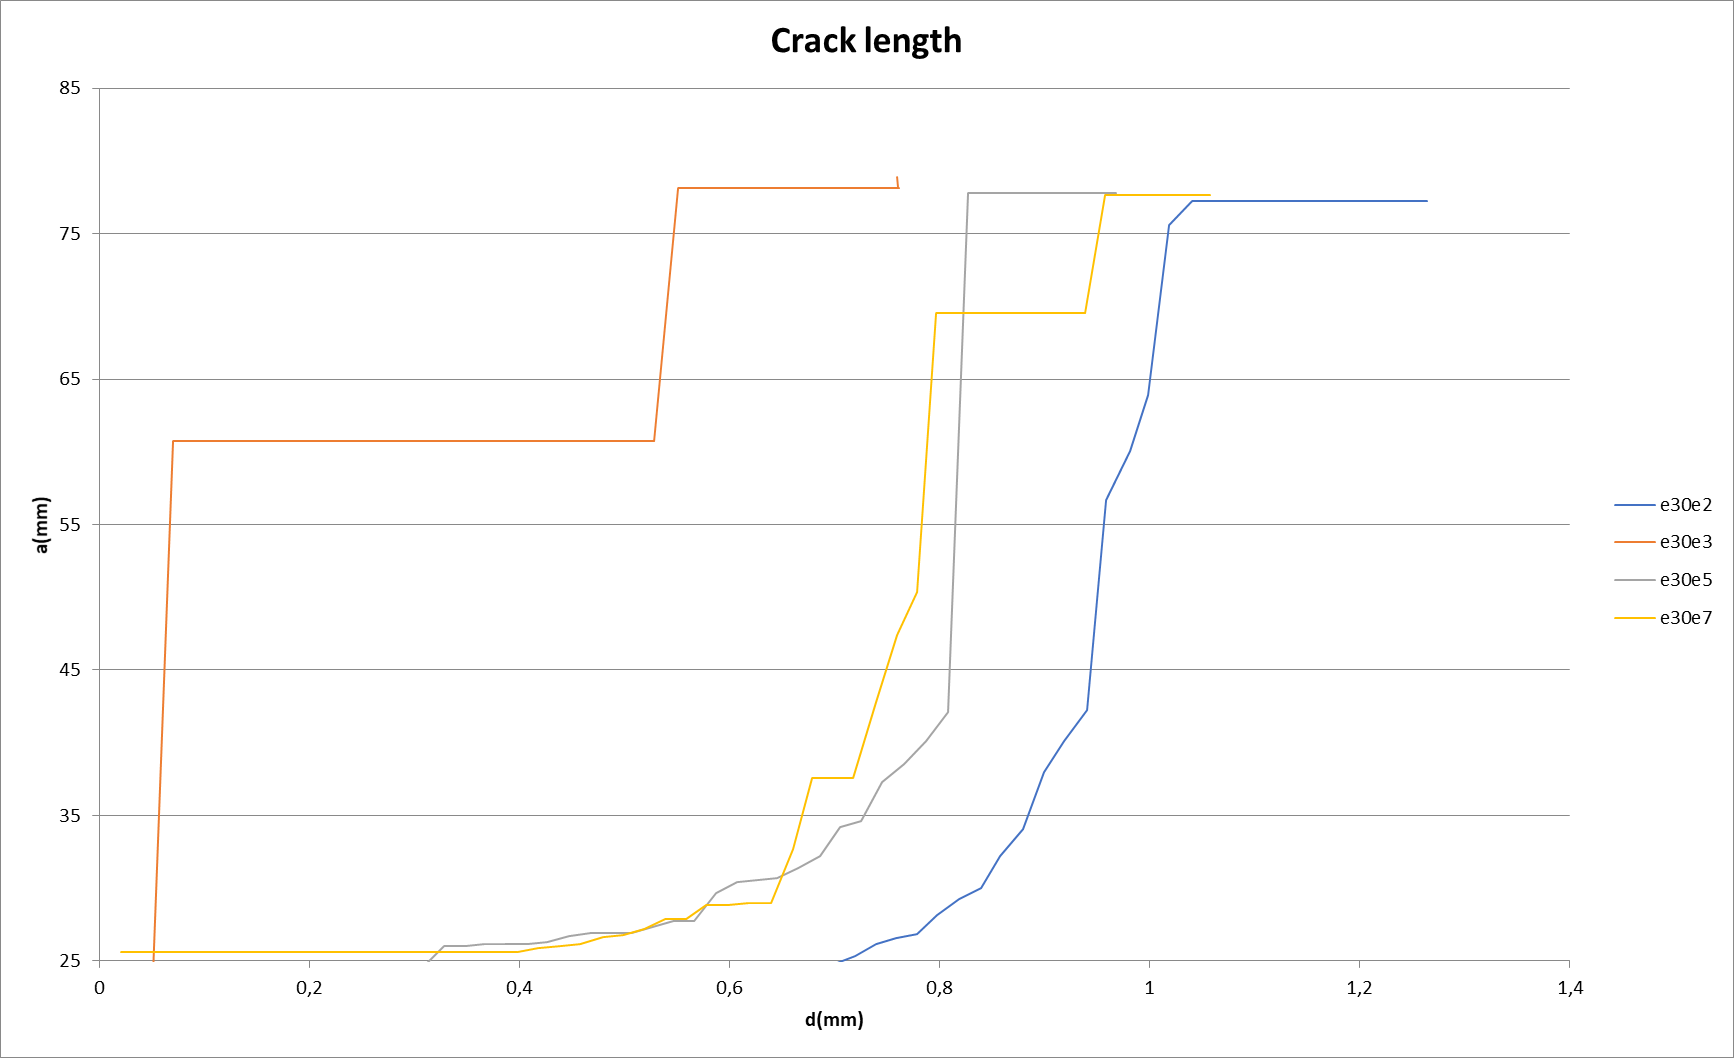
\includegraphics[width=13cm]{crack_30}
	\caption{Crack length evolution for 30°specimens.}
	\label{fig:crack_30}
\end{figure}

\subsection{Critical energy release rate}

Figures \ref{fig:G1_15} and \ref{fig:G2_15} depict the decoupled energy release rate for mixed-mode I+II at a 15° angle.
In terms of mode I, the maximum energy release rate attainment varies with respect to the crack length $a(t)$ for both mode I and mode II components. Specifically, the mode I component reaches $G_\text{Imax}$ within the range of crack lengths between 52 and 80 mm. Conversely, the mode II component achieves $G_\text{IImax}$ when the crack length falls within the 38 to 64 mm range. The disparity observed in the values of $a(t)$ for $G_\text{Imax}$ and $G_\text{IImax}$ can be attributed to the influence of CTOD measurements, which differ in their sensitivity to crack propagation between the two modes.
Furthermore, it is noteworthy that the energy release rate curves exhibit a plateau-like behaviour, aligning with the anticipated shape for energy release rate plots. This characteristic indicates the stability provided by the design of the MMCG specimen, which enhances resistance near the crack tip and contributes to the overall stability of the energy release rate.

\begin{figure}[htp]
	\centering
	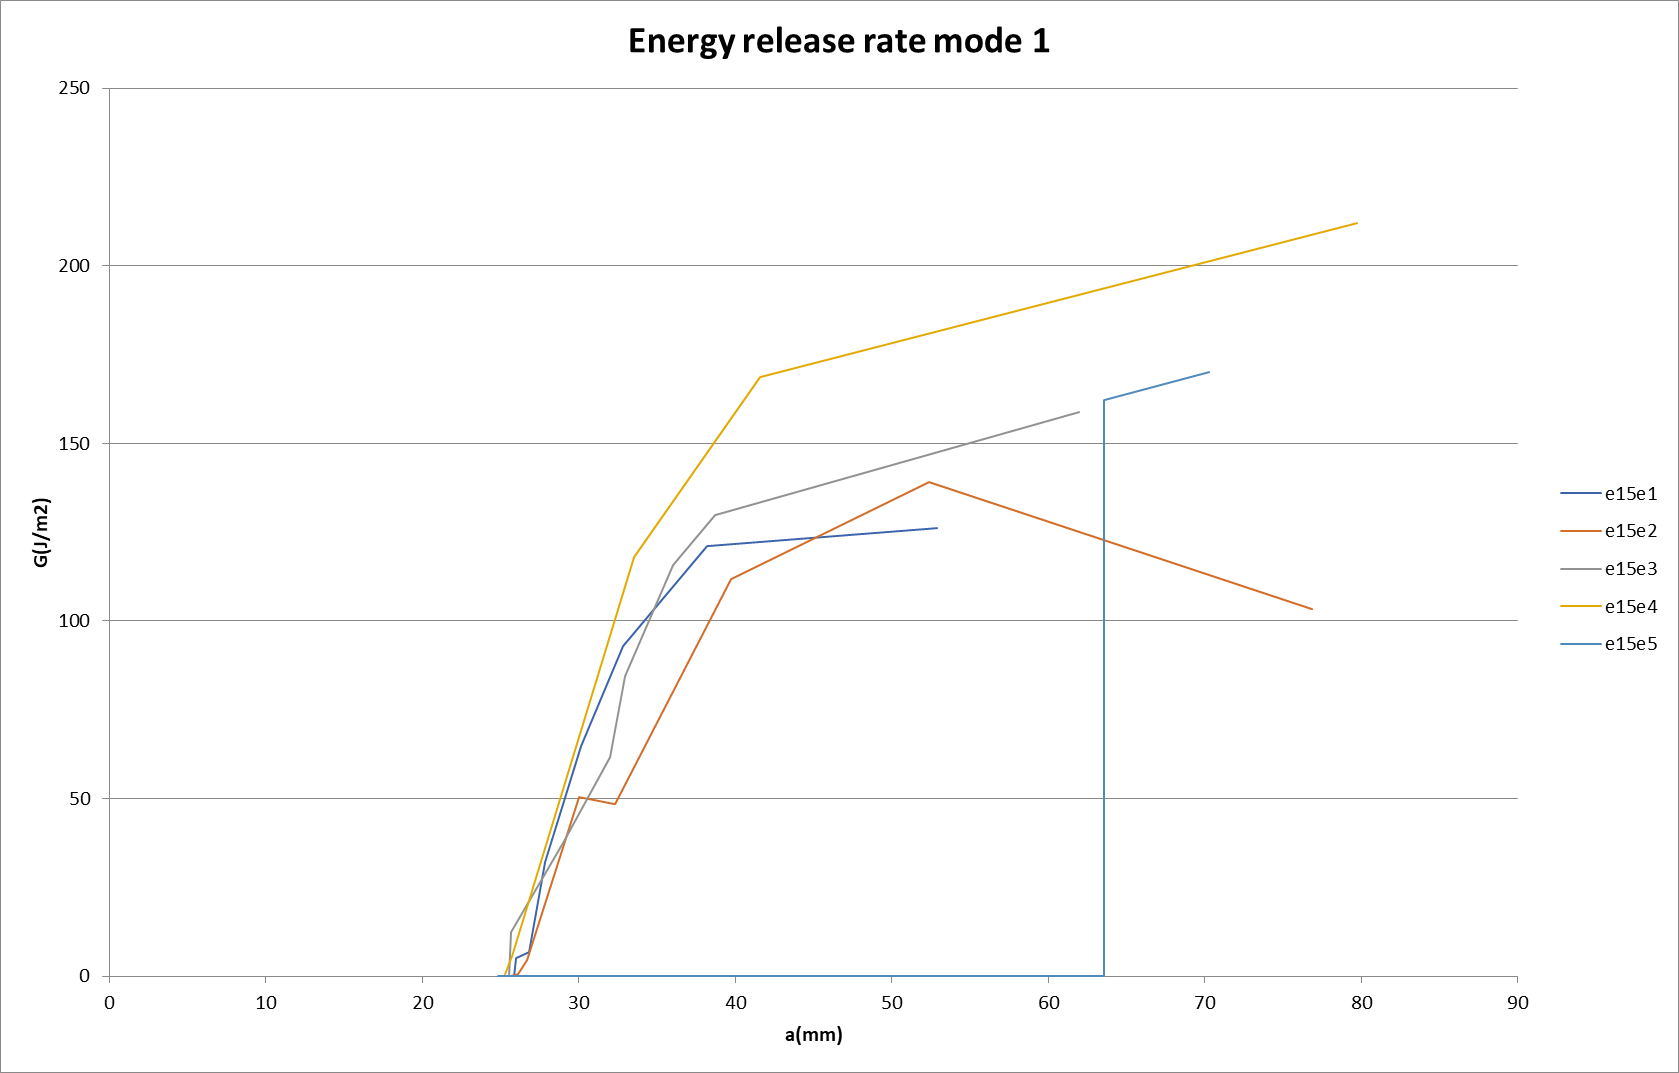
\includegraphics[width=12.5cm]{G1_15}
	\caption{Energy release rate as a function of crack length for 15°; mode I component.}
	\label{fig:G1_15}
\end{figure}

\begin{figure}[htp]
	\centering
	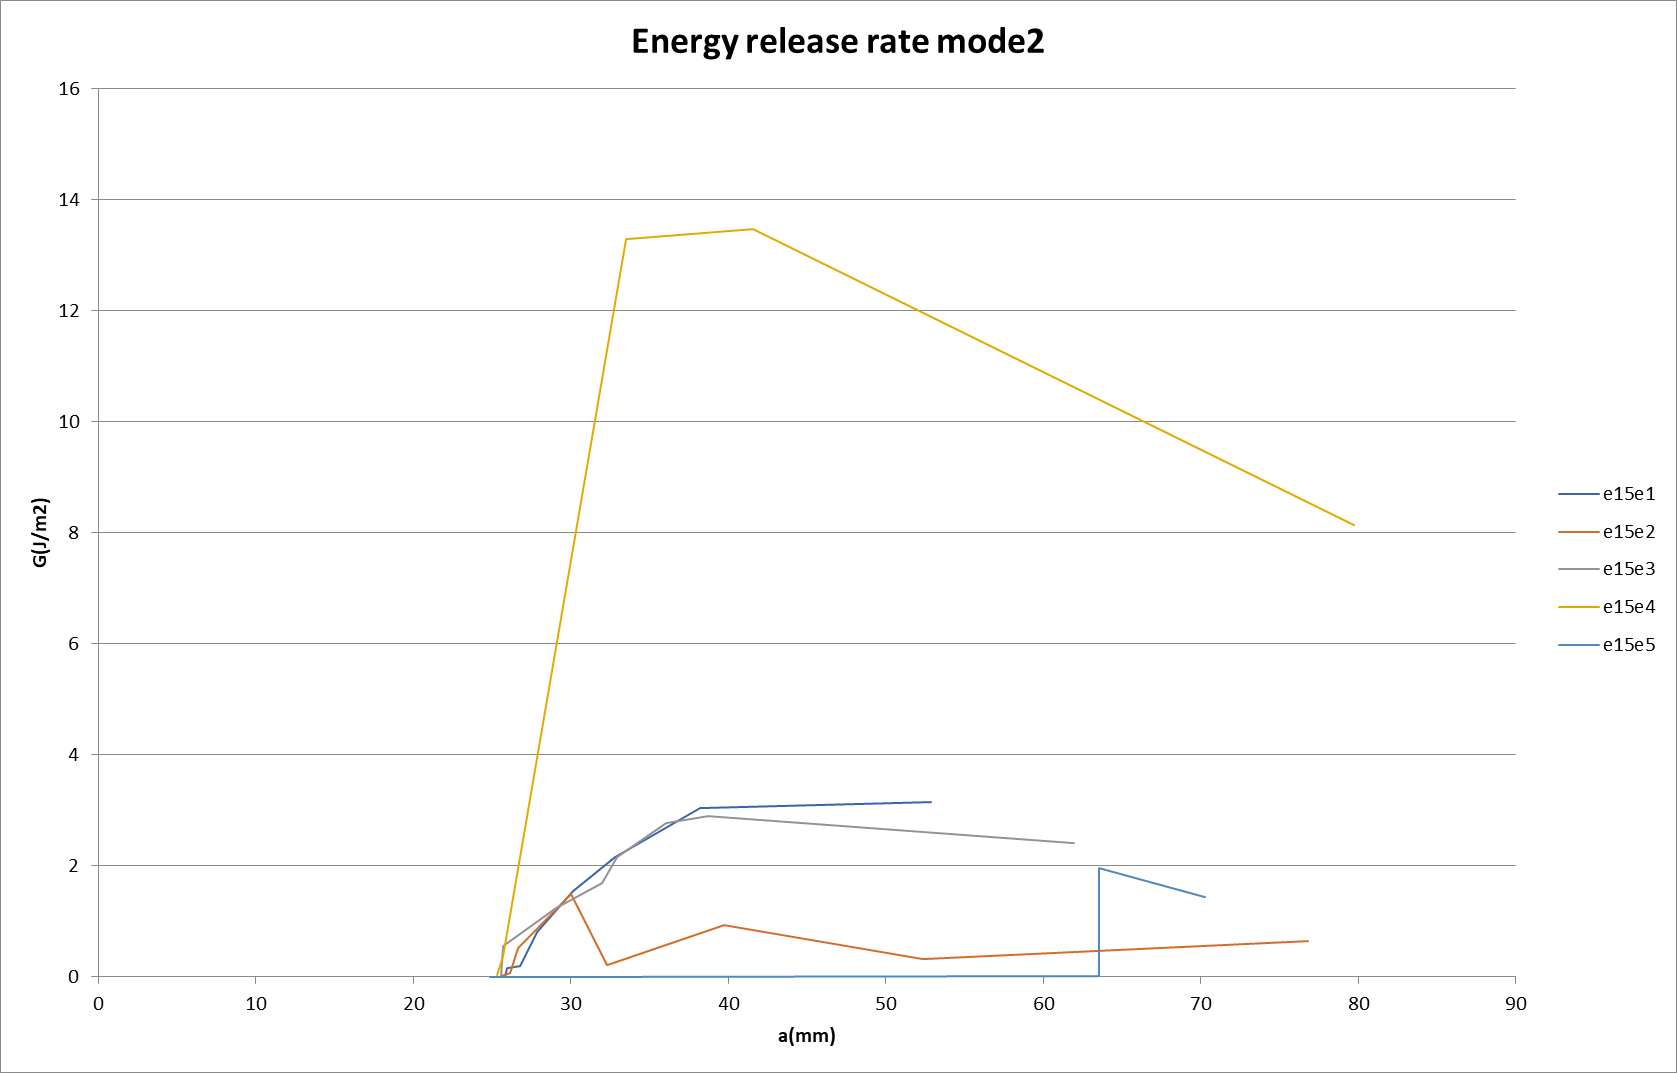
\includegraphics[width=12.5cm]{G2_15}
	\caption{Energy release rate as a function of crack length for 15°; mode II component.}
	\label{fig:G2_15}
\end{figure}

Table \ref{fig:tableG15} presents the maximum values of $G_\text{I}$ and $G_\text{II}$ for the 15° angle. The data highlights a distinct predominance of mode I over mode II. It is worth noting that the standard deviation for mode I is relatively low, indicating consistency in the results. However, for mode II, the standard deviation appears to be relatively higher, primarily influenced by the value of $G_\text{II}$ obtained from e15e4 specimen.

\begin{table} [H]
	\centering
	\begin{tabular}{ccccccccc}
		\toprule % horizontal line at the top of the table
		&  & e15e1 & e15e2 & e15e3 & e15e4 & e15e5 & Mean & Standard deviation\\\midrule
		& $G_\text{Imax}$ (J/m$^2$) & 126.21 & 139.19 & 158.93 & 212.07 & 169.98 & 161.28 & 33.09 \\
		& $G_\text{IImax}$ (J/m$^2$) & 3.15 & 0.93 & 2.90 & 13.48 & 1.95 & 4.60 & 5.01\\\bottomrule
	\end{tabular}
	\caption{$G_{max}$ values for Silver Fir specimens in mixed mode for 15°}
	\label{fig:tableG15}
\end{table}

Figures \ref{fig:G1_30} and \ref{fig:G2_30} show the decoupled energy release rate for the mixed mode with 30° angle. We can see that for values of $a(t)$ between 42 and 78 mm, the mode I component reaches $G_\text{max}$, whereas for the mode II component, for values of $a(t)$ between 32 and 61 mm, the mode 2 part reaches $G_\text{IImax}$.

\begin{figure}[htp]
	\centering
	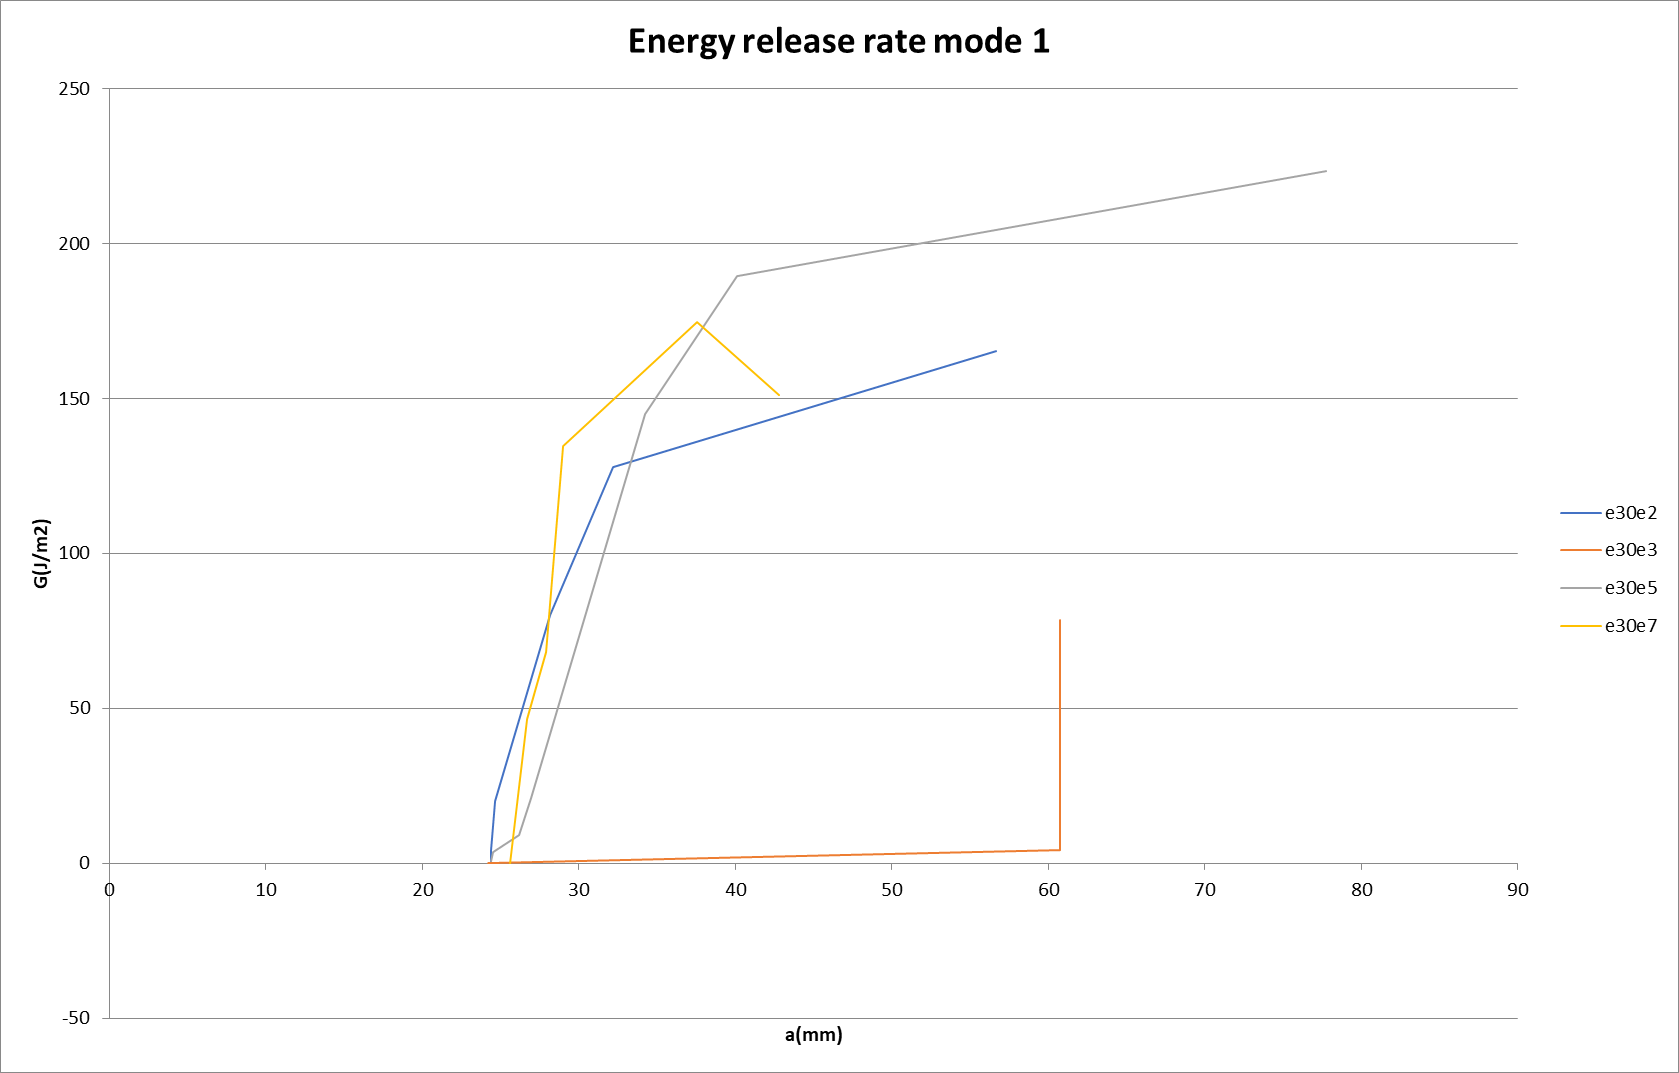
\includegraphics[width=12.5cm]{G1_30}
	\caption{Energy release rate as a function of crack length for 30°; mode I component.}
	\label{fig:G1_30}
\end{figure}


\begin{figure}[htp]
	\centering
	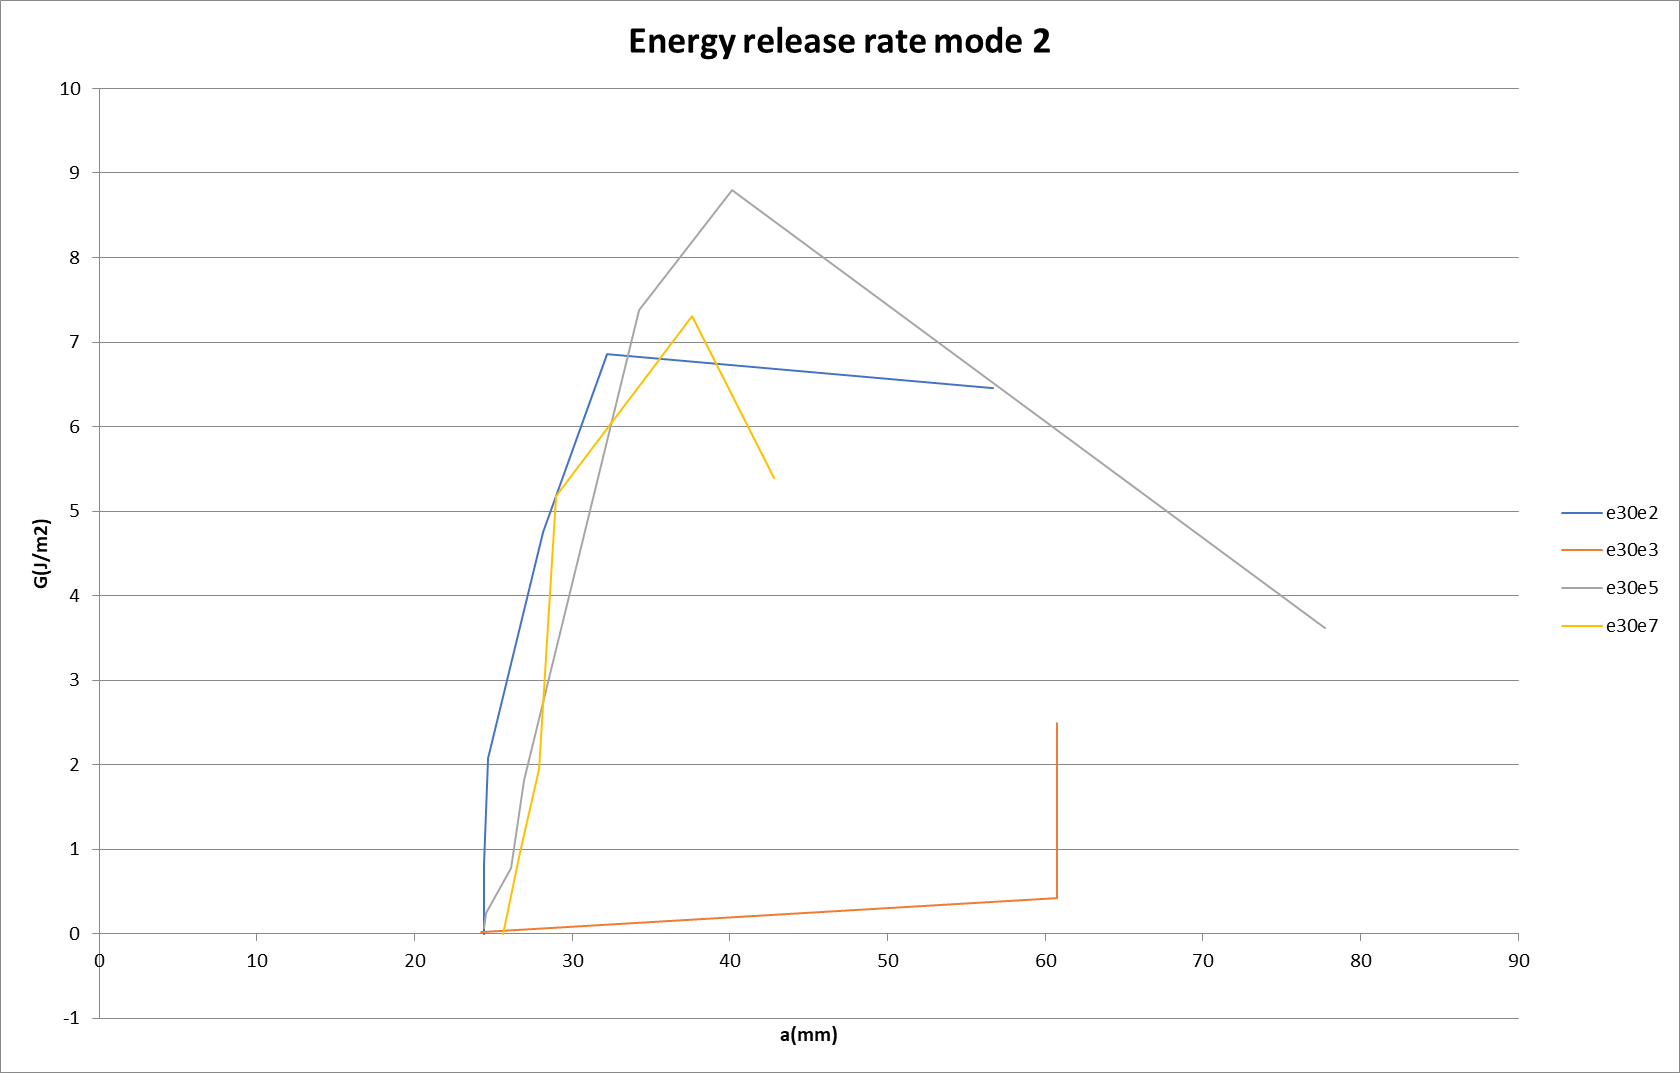
\includegraphics[width=12.5cm]{G2_30}
	\caption{Energy release rate as a function of crack length for 30°; mode II component.}
	\label{fig:G2_30}
\end{figure}

Table \ref{fig:tableG30} gives the maximum values of $G_\text{I}$ and $G_\text{II}$ for 30° angle. The values are similar to those for 15° angle, but there is a slight increase in $G_\text{II}$.

\begin{table} [H]
	\centering
	\begin{tabular}{cccccccc}
		\toprule % horizontal line at the top of the table
		&  & e30e2 & e30e3 & e30e5 & e30e7 & Mean & Standard deviation\\\midrule
		& $G_\text{Imax}$ (J/m$^2$)  & 165.38 & 78.58 & 223.31 & 174.74 & 160.50 & 60.23 \\
		& $G_\text{IImax}$ (J/m$^2$) & 6.86 & 2.49 & 8.80 & 7.31 & 6.37 & 2.71\\\bottomrule
	\end{tabular}
	\caption{$G_{max}$ values for Silver Fir specimens in mixed mode for 30°.}
	\label{fig:tableG30}
\end{table}

\section{Discussion of the results}

\subsection{Data analysis and comparison}

Table \ref{fig:Comparison_angle} shows the average $G_\text{max}$ values for the different mixing angles. It also shows the breaking force applied to the specimen for the 3 angles. The differences between modes I and II are compared.

\begin{table} [H]
	\centering
	\begin{tabular}{ccccccccc}
		\toprule % horizontal line at the top of the table
		&  & 0° & 15° & 30° \\\midrule
		& $G_\text{Imax}$ (J/m$^2$)  & 170 & 161.28 & 160.5  \\
		& $G_\text{IImax}$ (J/m$^2$) & 0 & 4.6 & 6.37 \\
		& $G_\text{IImax} - G_\text{Imax}$ (J/m$^2$) & 170 & 156.68 & 154.13 \\
		& $P_\text{max}$, (N) & 395.8 & 433.8 & 457.3 \\\bottomrule
	\end{tabular}
	\caption{Comparison of the energy release rate as a function of the mixing angle.}
	\label{fig:Comparison_angle}
\end{table}

Depending on the mixing angles considered, there is a slight decrease in the disparity between mode I and mode II as the mixing angle increases. The results yield the following insights upon analysing the tests conducted for different mixing ratios. Across all studied mixing angles, the share of mode I consistently exceed that of mode II.

The applied force leading to specimen failure increases with higher mixing angles. This phenomenon can be attributed to the maximum resistance observed when the load is parallel to the fibres.
In terms of energy release rate, the values for mode I decrease with increasing mixing angles, while the values for mode II increase, consistent with the findings of Odounga (2018). However, this variation is relatively small, and conducting tests with larger mixing angles would provide a better assessment of this hypothesis.

The difference between $G_\text{I}$ and $G_\text{II}$ diminishes as the mixing angle increases, thereby justifying the complete decoupling of mixed failure modes. There is an observable decreasing trend in the difference between $G_\text{I}$ and $G_\text{II}$.
In \citet{Odounga2018phd} results, the crack opening values along the $x$ and $y$ axes tend to converge as the mixing angle approaches 45 degrees. In mixed mode scenarios, the crack opening displacement is no longer one-dimensional due to the specimen being subjected to an angled stress that induces the coexistence of both modes, resulting in a projection along both axes of the crack opening. Determining the two components, u and v, enables the calculation of $G_\text{I}$ and $G_\text{II}$, effectively decoupling the two modes. The disparity between the values of the two modes is most significant at smaller mixing angles. According to \citet{Odounga2018phd}, this difference decreases until a mixing angle of 45 degrees, at which point it becomes minimal. Between 0 and 45 degrees, mode I surpasses mode II. It is likely that after a mixing angle of 45$^\circ$, mode II is expected to dominate over mode I.

Furthermore, the obtained results align with those of \citet{MoutouPitti2008}, who conducted experiments with Douglas fir specimens. For a mixing angle of 15 degrees, they experimentally obtained $G_\text{Imax}$=250 J/m2 and $G_\text{IImax}$=8 J/m2. Similarly, for a mixing angle of 30 degrees, they obtained $G_\text{Imax}$=270 J/m2 and $G_\text{IImax}$=18 J/m2, which closely resemble the results obtained in this study.
However, it is important to note that the values reported by Odounga (2018) for mixed-mode differ, as he obtains GI values on the order of $10^2 J/m^2$.

\subsection{Difficulties and improvements}

Other researchers can continue the study, and numerous improvements can be made. The specimens' preparation, content, and shape all need to be carefully controlled. Indeed, even while the thickness, precrack, and other characteristics that we measured are taken into consideration in the calculations and tests, these are still approximations. Therefore, having very slight bias in all of these parameters has an impact on the final results.

One problem with this work was also the raw data from the servo-hydraulic press device. Indeed, as explained, an offset was applied to the P-delta curve to avoid negative values that made no sense. It was decided to shift P with its minimal value to account for the preload. In some situations, the last index of P was lower than the first index and that the machine appears to be able to move freely for the last indices of P without any change in the force P. Therefore, we decided that this delta P matched the preload. However, in some cases, the machine cannot be seen to move freely without a change in the force P for the last indices of P. As a result, the preload is sometimes underestimated because there is some preload tension that cannot be measured.
By roughly estimating this first load, all the results are slightly truncated and there is an impact on the other parameters. Incorrect values have an impact on these calculations since the load P is required to determine Compliance and the energy release rate. The square factor applied to the load parameter has a special impact on G. Before using the hydraulic press, it is essential to check the load in order to solve this issue.

Another problem is illustrated by figure \ref{fig:Crack_junction}. The MMCG specimen has a crack at the connection fillet. Indeed, among the difficulties encountered, the brittleness of the specimens at the level of the connection fillet is precisely the one that caused the most problems. It is for this reason that several tests were not used. Three tests with a 30° angle and one test with a 45° angle broke at the connection fillet. One specimen at 0° did not crack at the initial crack tip and finally one specimen broke because the machine stopped abruptly during the test because it was overheating. In conclusion, fourteen tests were successful and it was only possible to analyse for the 0°, 15° and 30° angles. In future tests, it will be important to reinforce the specimen in some areas.

\begin{figure}[htp]
	\centering
	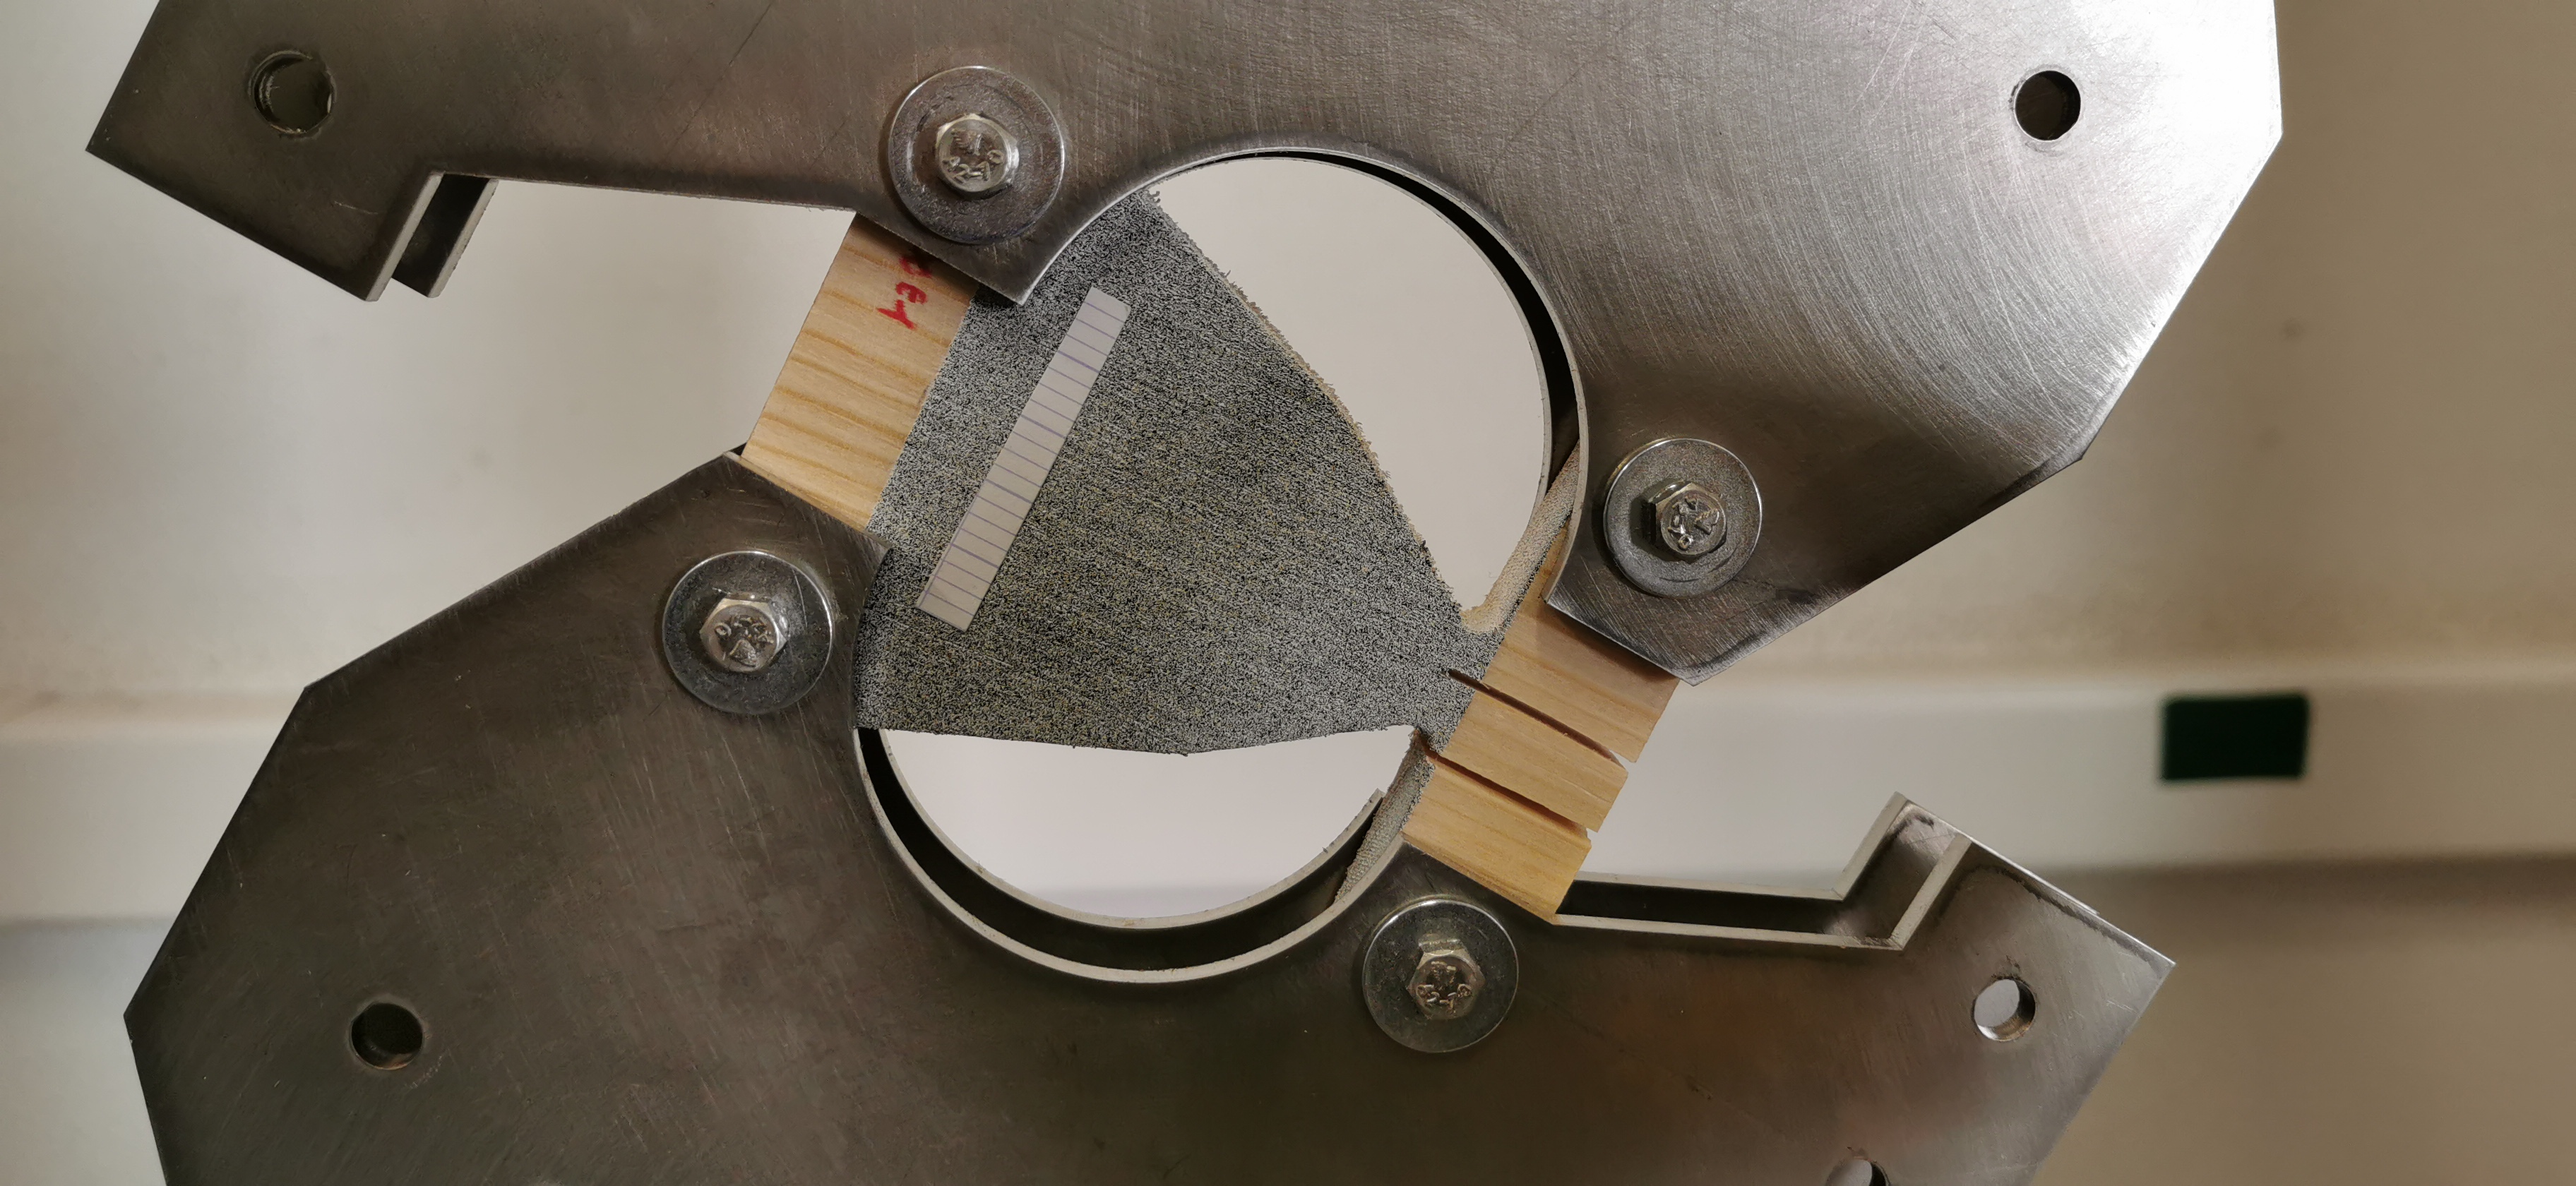
\includegraphics[width=12cm]{Crack_junction}
	\caption{Fracture issues encountered at the connection fillets.}
	\label{fig:Crack_junction}
\end{figure}

Various methods of calculating $G$ were tested. It was considered to use compliance as a function derived from the crack length. In order to make a(t) smoother, we decided to take only the indices of $a(t)$ when propagation occurs. In other words, we removed the duplicate $a(t)$. We then tried to interpolate a(t) with different functions. However, the interpolated functions could have fit better at all points.
Finally, it was decided to use the same methodology as \cite{MoutouPitti2008}, \cite{Mambili2018} and  \cite{Odounga2018phd}, i.e. to take only the indices where there is a critical force signifying a crack propagation and calculating $\Delta c$/$\Delta a$ between the starting point and the point considered for all the critical forces.

In this study, comparing the results obtained with the Abaqus software was impossible. This comparison could provide a better understanding of the behaviour of wood and enable the results to be verified. A colleague at the university who is also doing a thesis master's degree is currently working on the finite element method to compare the results obtained in this work with those he will obtain numerically. In addition, it might be interesting to carry out more tests with softwood specimens in mode I and mixed mode, since only fourteen specimens were tested in this study.
Finally, a solution to prevent the specimens from breaking at the fillet connection might be worth considering.

\section{Conclusion}

This chapter investigated Silver Fir's crack behaviour under mixed-mode I+II conditions using MMCG specimens. The Arcan fixture was employed to conduct fracture tests with specimen orientations of 15° and 30°. Unfortunately, tests at a 45° angle were not feasible due to multiple specimen failures at the fillet connection. The decoupling of modes allowed for determining the contributions of modes I and II. Detailed strain maps were generated, and results on force-crack opening displacement relationships and energy release rates as a function of crack length were presented. The findings from the compliance method, which involved calculating energy release rates at specified displacements, revealed a predominance of mode I over mode II. Furthermore, this predominance was observed to diminish as the mixing angle increased.